\documentclass[paper=a4, fontsize=11pt]{scrartcl}

\usepackage[T1]{fontenc}
\usepackage{fourier}
\usepackage[utf8]{inputenc}

\usepackage[english]{babel}															% English language/hyphenation
\usepackage[protrusion=true,expansion=true]{microtype}	
\usepackage{amsmath,amsfonts,amsthm} % Math packages
\usepackage[pdftex]{graphicx}	
\usepackage{url}
\usepackage{abstract}
\usepackage{tabularx}
\usepackage{float}

%%% Custom sectioning
\usepackage{sectsty}
\allsectionsfont{\centering \normalfont\scshape}

%%% Custom headers/footers (fancyhdr package)
\usepackage{fancyhdr}
\pagestyle{fancyplain}
\fancyhead{}											% No page header
\fancyfoot[L]{}											% Empty 
\fancyfoot[C]{}											% Empty
\fancyfoot[R]{\thepage}									% Pagenumbering
\renewcommand{\headrulewidth}{0pt}			% Remove header underlines
\setlength{\headheight}{13.6pt}

%%% Equation and float numbering
\numberwithin{equation}{section}		% Equationnumbering: section.eq#
\numberwithin{figure}{section}			% Figurenumbering: section.fig#
\numberwithin{table}{section}				% Tablenumbering: section.tab#

%%% Maketitle metadata
\newcommand{\horrule}[1]{\rule{\linewidth}{#1}} 	% Horizontal rule

\title{
		%\vspace{-1in} 	
		\usefont{OT1}{bch}{b}{n}
		\normalfont \normalsize \textsc{Luleå University of Technology} \\ [25pt]
		\horrule{0.5pt} \\[0.4cm]
		\huge Algorithms and Data Structures - Laboration 1 \\
		\horrule{2pt} \\[0.5cm]
}
\author{Course: D0012E \\ \\ 
		\normalfont 								\normalsize
        Marcus Lund (amuulo-4) \\\normalfont\normalsize Edvin Åkerfeldt (edvker-4)\\\normalfont\normalsize Samuel Karlsson (samkar-4)\\[-3pt]		\normalsize
        \today
}
\date{}

%%% Begin document
\begin{document}
\maketitle
\centerline{First submission.}
\begin{figure}[h!]
  \centering
    
\includegraphics[width=1\textwidth]{algorithm}
\end{figure}
\newpage

\begin{abstract}
We have implemented the two sorting algorithms, insertionsort and binsertionsort. Binsertionsort is a variation of insertionsort where you use a binary search to find the place for any new number. The regular insertionsort use linear search instead of binary search. We also implemented a merge sort that divide the array into sub-arrays of size equal or less the $k$ ($k$ is a positive integer). The sub-arrays are then sorted by insertionsort or binsertionsort. Finally we merge the sorted sub-arrays back together using standard merge sort algorithm.

We compared the run-times when using insertinonsort and binsertionsort. We found that insertionsort's runtime increases logarithmic while the binsetrionsort takes less time, it also resembles a logarithmic function but it increases much slower. 
The runtime of insertionsort increases by a factor of two for each time $k$ has been doubled. This is dune because of the merge sort that split the array in half and give insertionsort twice the amount of work. In small array sizes, insertionsort may be faster than binsertionsort. These cases has an array of a very small size. Both algorithms runs in $\theta(nk + n\lg(\frac{n}{k}))$ worst case time. Generally, binsertionsort is much faster than insertionsort in average case.

\end{abstract}

\tableofcontents
\newpage

\section{Introduction}   %might wana rewrite this part
We began by looking into how the two algorithms would be implemented. Then both algorithms were then implemented in our language of choice, Python. The first implementation was sloppy and slow, but after a few improvements to the code (reducing function calls and comparisons) we managed to get a faster and better implementation overall while keeping the functionality of the algorithms intact. 

\section{Language}
We choose Python as our language of choice because of the easy implementation of array splitting. Another contributing factor was the general easy to use syntax. We are aware of the fact that it is ugly compared to other languages due to the fact that there is little structure in the code syntax itself. Although we decided to choose this language we are also aware of it's drawbacks, such as: slow execution time compared to C++ or java, low recursion depth compared to other languages and the lack of variable declarations (implies more error checks). All together we decided that Python was a good choice due to the big advantages the array splitting gives in terms of easy implementation.

\section{Implementation}
By following the convention of merge sort, we recursively split the array into k-sized segments by splitting the array in half and continued until each segment is of size k or less. These segments are then sorted using either insertionsort or binsertionsort. The sorted segments are then merged using the standard merging algorithm.

\section{Test procedure}
We decided to run the first tests several times and take the average values from the results of each k and array size. With a larger $k$ and array we ran the tests fewer times to reduce the total runtime.  

The test we conducted were based a single array generated for each arraysize with the numbers in the array randomly generated from 0 to $10^6$. If we would have used a fixed array we would get the same results each run. We wanted to test different arrays and compare the average to get as close real-life results as possible.

\section{Result}
We decided to do four tests, one with an array of size $1000$ where the $k$ values ($k$ is a positive integer) are $1-1000$ with the interval $1$ (graf \ref{graf1000}). The second test was with an array with the size $50,000$ and the $k$ values were $100-50,000$ with the interval $1000$ (graf \ref{graf50}). The third test was with an array of size $200,000$ and the $k$ values were $1-200,000$ with logarithmic intervals (graf \ref{graf200}). The final test was with an array size of $2,000,000$ and the $k$ value where $1-500,000$ with a logarithmic intervals (graf \ref{graf524}).



As we can see in the graph \ref{graf50}, the time is increasing in steps. The increasing of runtime appears in logarithmic intervals. Both insertionsort and binsertionsort experience increasing runtime at the same k-value, though the amount of timeincrease is different for each function./////////////////////////


\begin{figure}[ht!]
\centering
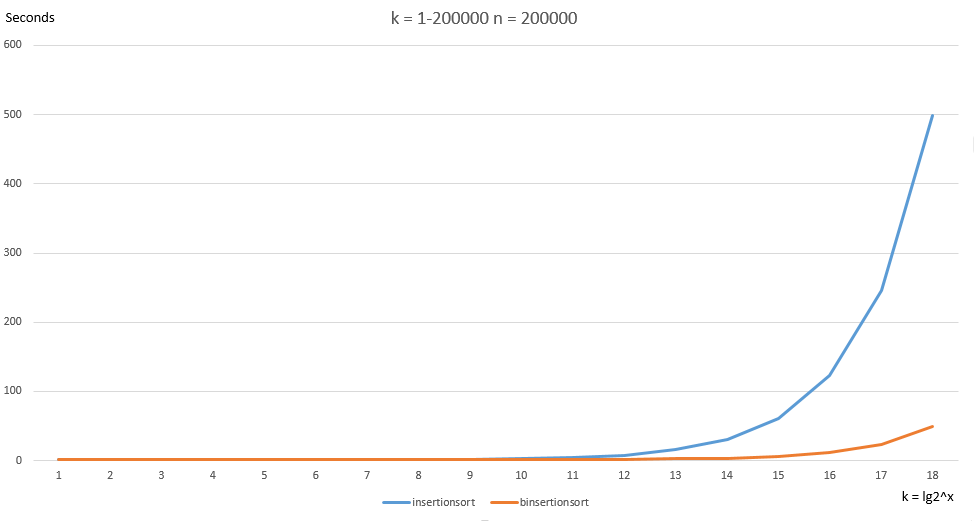
\includegraphics[width=150mm]{graf_lg1-200000.png}
\caption{A graph of a test with an array size of $200,000$ and the $k$ value various between $1$ and $200,000$ where the time measured
 for every logarithmic increse of $k$. \label{graf200}}
\end{figure}

In the graph \ref{graf200} where $k$ increased logarithmic-wise, we noticed that the time was increasing exponentially when $k$ grew into larger $k$ values.

Both algorithms were increased when $k$ passed a exponential power of $2$.

\subsection{Insertionsort}

From the grafes is it clear that insertionsort gets rely bad wen deling wid huge data sets. From graf \ref{graf200} and graf \ref{graf524} is it clear that the time get redicules hige.

A intresting thing that can be sen clearly in graf \ref{graf50} thet the time dubels in logaritmi intervals. This geiv as the nice star loging graf.

\subsection{Binsertionsort}
Ass insertionsort seam binsertionsort to incrise i logaritmik intervals, but binsertionsort do not increse as mutch. Sens binsertionsort splitt the array ín tow multible times is it lodgik tht it increses wen an pasing the line of a power of $2$, becos it the neds to split the array in tow equal long arrays that prevues wer the howl array.



\newpage

\subsection{Graphs}

\subsubsection{Test 1, K $1$-$1000$}

\begin{figure}[H]
\centering
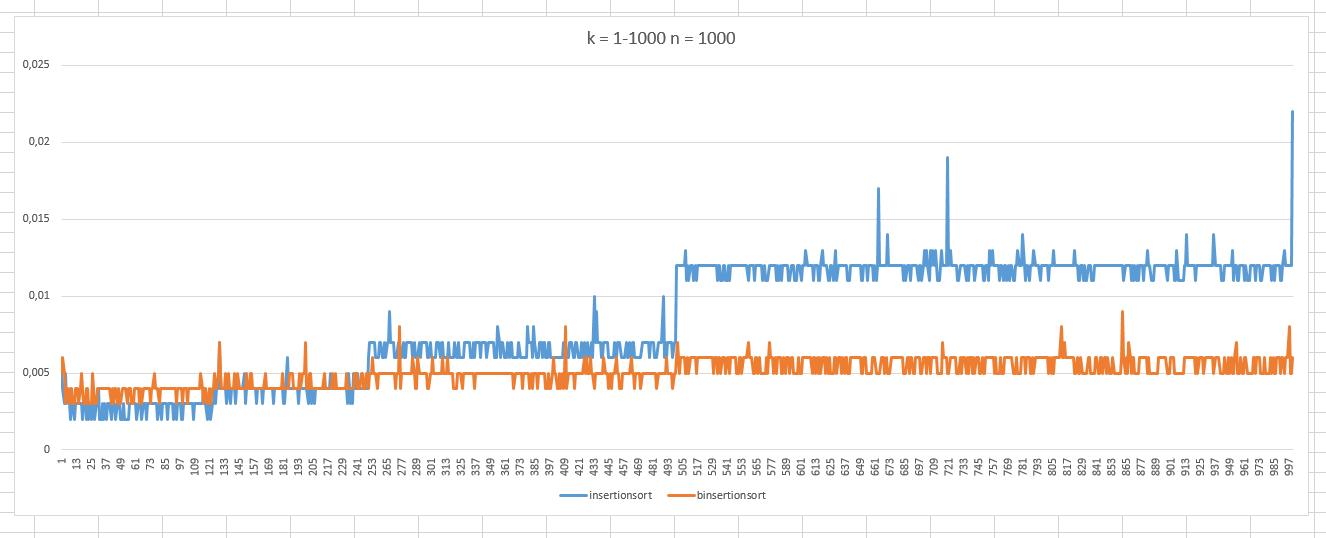
\includegraphics[width=150mm]{k1-1000N=1000.png}
\caption{A graf of a test whith a array size of $50 000$ and the $k$ walue warius betwem $100$ and $50 000$ wher the time metserd ouns evry $1000$. \label{graf1000}}
\end{figure}

Here we see that small values are in some cases worse with binsertionsort. There is however a volume in witch binsertionsort switches as the better choise than regular insertionsort. Although the arraysize is only $1000$, we see the small difference. We decided to run even bigger arrays with values from $1$ to $2 000 000$.

\subsubsection{Test 2, K $100$-$50 000$}

\begin{figure}[H]
\centering
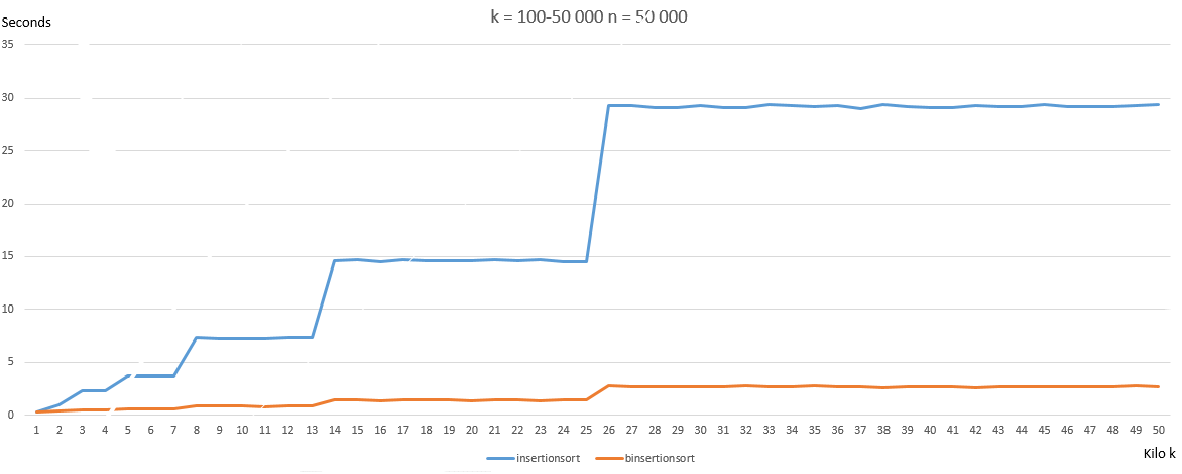
\includegraphics[width=150mm]{graf100-50000.png}
\caption{A graf of a test whith a array size of $50 000$ and the $k$ walue warius betwem $100$ and $50 000$ wher the time metserd ouns evry $1000$. \label{graf50}}
\end{figure}

Here we can figure \ref{graf50} ease see the increase of both algorithms and the difference of the two. while insertionsort quickly increases, binsertionsort doesn't increase nearly as much. This is when K=$100$-$50 000$ and an array of size $50000$.

\subsubsection{Test 3, K $1$-$524 288$}

\begin{figure}[H]
\centering
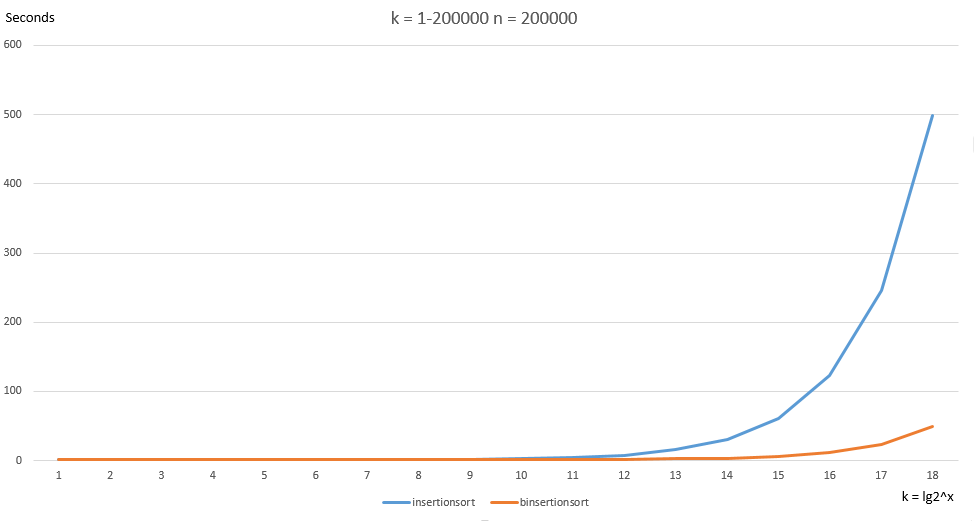
\includegraphics[width=150mm]{graf_lg1-200000.png}
\caption{A graf of a test whith a array size of $200 000$ and the $k$ walue warius betwem $1$ and $524 288$. \label{graf524}}
\end{figure}

\begin{table}[H]
\begin{center}
\begin{tabular}{|l|l|l|}	
    \hline
    K				& insertionsort   & binsertionsort \\ \hline
    1				& 15.2799999714   & 16.0329999924 \\
    2				& 13.4079999924   & 13.9700000286 \\
    4				& 12.1639997959   & 13.2150001526 \\
    8				& 11.5429999828   & 12.6840000153 \\
    16				& 10.5320000648   & 12.4670000076 \\
    32				& 10.8150000572   & 13.3180000782 \\
    64				& 11.7960000038   & 14.0509998798 \\
    128				& 14.1679999828   & 14.9419999123 \\
    256				& 19.7150001526   & 16.2039999962 \\
    512				& 30.8680000305   & 17.6510000229 \\
    1024			& 53.9000000954   & 19.7840001583 \\
    2048			& 100.339999914   & 23.3710000515 \\
    4096			& 194.943000078   & 30.0620000362 \\ 
    8192			& 384.326999903   & 44.7890000343 \\
    16384			& 752.871000051   & 79.0769999027 \\ 
    32768			& 1526.60899997   & 152.967000008 \\ 
    65536			& 3139.0769999    & 303.378000021 \\
	131072			& 6468.52200007   & 667.940000057 \\
	262144			& 13433.013       & 1536.90400004 \\
	524288			& 25904.4170001   & 5946.81500006 \\
    \hline
\end{tabular}
\end{center}
\caption{K from $1$ to $524 288$, Array size $2 000 000$}
\label{table01}
\end{table}

The graph \ref{graf524} and its values of table \ref{table01} is generated by starting with K=$1$ and array size=$2 000 000$. The values in the array are between $1$ to $2 000 000$. In this test we double the K value each step and watching the diffrences in boath algorithms. The results are ploted in graph \ref{graf524}.
The table shows us that insertionsort doubles its time to sort by a factor of two while binsertionsort takes less time but also starts to (almost) double its values at a larger K value.

\section{Discussion}
The results we got were not surprising. We suspected in pre-test that insertionsort was worse than binsertionsort. Though we had not foreseen that there would be such clear steps in the graphs (clear seen in graf \ref{graf50}). Although it was surprising, when you think about it it is fairly obvious that it should be such clear steps due to the algorithms. 

When we look at merge sort we can clearly see this. For example, an array split into segments of $4$ will take, roughly, half the time compared to an array split into segments of $8$. If the array size has $8$ elements and should be split one time, we get two arrays that has the length of $4$ each . This means that we have two arrays has the length of $4$ and therefore takes twice the time to execute. It was a bit surprising that binsertionsort increased runtime so slowly however.

Our implementation and choice to use random arrays may had an impact on our results. This may cause inconsistent values in our graphs. The operating system will most likely have an influence on the test result due to other process running in the background. We have minimised the risk of that by using a computer that had enough computer power to not be interrupted. The system ran test for a period of 72 hours without any other process than windows and the test. We where able to find a trend that where similar to the function $\theta(nk + n\lg(\frac{n}{k}))$.

$\theta(nk + n\lg(\frac{n}{k}))$ is the maximum allowed time for the algorithm to execute. $\theta(n\lg(\frac{n}{k}))$ is when spiting the array into $k$ sized arrays and $\theta(nk)$ is for sorting the arrays while merging them back together. $\theta(nk)$ is equal to the runtime of insertionsort for all sub-arrays.

The most contributing factor to these algorithms are the sorting section. Because of the array size could be big, the merge would split the size into several sub-arrays and therefore takes shorter time compared to the sorting part of the program.

In the lab we learned that python is a really bad optimised language. When we talked to friends about their solution and their array sizes, our size was smaller compared to theirs. Yet their algorithms where faster as well. We conclude that it was because of the different performances of other languages. The longest test we ran took roughly 7 hours and it had an array size of only $2,000,000$. If the algorithms is to be analysed in bigger datasets it would be necessary to rewrite them in a different language.


%%% End document
\end{document}
